\documentclass{article}\usepackage[]{graphicx}\usepackage[]{xcolor}
% maxwidth is the original width if it is less than linewidth
% otherwise use linewidth (to make sure the graphics do not exceed the margin)
\makeatletter
\def\maxwidth{ %
  \ifdim\Gin@nat@width>\linewidth
    \linewidth
  \else
    \Gin@nat@width
  \fi
}
\makeatother

\definecolor{fgcolor}{rgb}{0.345, 0.345, 0.345}
\newcommand{\hlnum}[1]{\textcolor[rgb]{0.686,0.059,0.569}{#1}}%
\newcommand{\hlsng}[1]{\textcolor[rgb]{0.192,0.494,0.8}{#1}}%
\newcommand{\hlcom}[1]{\textcolor[rgb]{0.678,0.584,0.686}{\textit{#1}}}%
\newcommand{\hlopt}[1]{\textcolor[rgb]{0,0,0}{#1}}%
\newcommand{\hldef}[1]{\textcolor[rgb]{0.345,0.345,0.345}{#1}}%
\newcommand{\hlkwa}[1]{\textcolor[rgb]{0.161,0.373,0.58}{\textbf{#1}}}%
\newcommand{\hlkwb}[1]{\textcolor[rgb]{0.69,0.353,0.396}{#1}}%
\newcommand{\hlkwc}[1]{\textcolor[rgb]{0.333,0.667,0.333}{#1}}%
\newcommand{\hlkwd}[1]{\textcolor[rgb]{0.737,0.353,0.396}{\textbf{#1}}}%
\let\hlipl\hlkwb

\usepackage{framed}
\makeatletter
\newenvironment{kframe}{%
 \def\at@end@of@kframe{}%
 \ifinner\ifhmode%
  \def\at@end@of@kframe{\end{minipage}}%
  \begin{minipage}{\columnwidth}%
 \fi\fi%
 \def\FrameCommand##1{\hskip\@totalleftmargin \hskip-\fboxsep
 \colorbox{shadecolor}{##1}\hskip-\fboxsep
     % There is no \\@totalrightmargin, so:
     \hskip-\linewidth \hskip-\@totalleftmargin \hskip\columnwidth}%
 \MakeFramed {\advance\hsize-\width
   \@totalleftmargin\z@ \linewidth\hsize
   \@setminipage}}%
 {\par\unskip\endMakeFramed%
 \at@end@of@kframe}
\makeatother

\definecolor{shadecolor}{rgb}{.97, .97, .97}
\definecolor{messagecolor}{rgb}{0, 0, 0}
\definecolor{warningcolor}{rgb}{1, 0, 1}
\definecolor{errorcolor}{rgb}{1, 0, 0}
\newenvironment{knitrout}{}{} % an empty environment to be redefined in TeX

\usepackage{alltt}

\usepackage{amsmath} %This allows me to use the align functionality.
                     %If you find yourself trying to replicate
                     %something you found online, ensure you're
                     %loading the necessary packages!
\usepackage{amsfonts}%Math font
\usepackage{graphicx}%For including graphics
\usepackage{booktabs}
\usepackage{hyperref}%For Hyperlinks
\usepackage[shortlabels]{enumitem}% For enumerated lists with labels specified
                                  % We had to run tlmgr_install("enumitem") in R
\hypersetup{colorlinks = true,citecolor=black} %set citations to have black (not green) color
\usepackage{natbib}        %For the bibliography
\setlength{\bibsep}{0pt plus 0.3ex}
\bibliographystyle{apalike}%For the bibliography
\usepackage[margin=0.50in]{geometry}
\usepackage{float}
\usepackage{multicol}

%fix for figures
\usepackage{caption}
\newenvironment{Figure}
  {\par\medskip\noindent\minipage{\linewidth}}
  {\endminipage\par\medskip}
\IfFileExists{upquote.sty}{\usepackage{upquote}}{}
\begin{document}
\vspace{-1in}
\title{Lab 5 -- MATH 240 -- Computational Statistics}

\author{
  Jackson Colby \\
  Colgate University  \\
  Mathematics  \\
  {\tt jcolby@colgate.edu}
}

\date{}

\maketitle

\begin{multicols}{2}


\section{Introduction}
This lab introduced us to new places to explore in \texttt{R} including different types of files and functions. We are introduced to two new packages, \emph{stringr} \citep{stringr} and \emph{jsonlite} \citep{jsonlite}. This lab focuses on working directories and importing files and extracting data. Additionally, the lab makes you clean and compile the data into a form where it is helpful to answer whatever research question you are trying to solve, which in this case is which of \emph{The Front Bottoms}, \emph{All Get Out} or \emph{Manchester Orchestra} had more of an impact on the song \emph{Allentown}.

\section{Methods}

\subsection{Lab 2}
For this lab we were given a folder to download, called MUSIC containing sub folders and .wav audio files. This part of the Lab consisted of two parts, Task 1 and Task 2 which the goal of them was to edit the .wav files to output a batfile.The second part of the lab we recieved .csv files where they contained json data which was to be cleaned and compiled to help answer the overall question. The \emph{stringr} package, \citep{stringr} was utilized to acheive this goal.

\subsection{Methods for Task 1}
The overall goal for this task was to work on directory skills, building a batch file for data processing. Through accessing a downloaded folder called MUSIC you could work with the .wav files inside. The end product is to build a batch file which can be used in Task 2 to help obtain information such as attributes about the songs.
\subsection{Methods for Task 2}
The overall goal for Task 2 was to process JSON Output and extract some information from the JSON file. This task helped set up for Lab 3 where we used the skills to help find attrubytes of the data using \emph{jsonlite} package \citep{jsonlite}.

\subsection{Methods for Lab 3}
The overall goal for this lab was to learn how to clean and compile data into data frames and csv files to be applied to the overall question of, Which band contributes most to the song? The song in question being \emph{Allentown}, which was composed by \emph{The Front Bottoms}, \emph{All Get Out}, and the \emph{Manchester Orchestra}. 

In order to acheive the goal of comparing the two bands on the song, packages for \texttt{R} such as \emph{stringr}, \citep{stringr} and \emph{jsonlite}, \citep{jsonlite} were used. The goal was to iterate through json data in a folder called \emph{EssentiaOutput}, and extract the data we wanted into a data frame. This data frame was then used to store some attributes about the song such as overall loudness and danceability, which could be used to compare and contrast songs. After manipulating the dataframe, we merged all the data we wanted to save into a new data frame with the \emph{streaming\_music\_extractor} and \emph{LIWC} and saved these into csv files where one contained all 180 songs other than \emph{Allentown}, and the other just contained \emph{Allentown}. 

\subsection{Methods for Lab 5}
This lab emphasized answering the overall question, which band contributed the most to the song \emph{Allentown} by using the library \emph{tidyverse}, \citep{tidyverse}. Through functions such as \texttt{group\_by(), summarize(), and mutate()}, a new data set was created that stored data for all the features of the averages for each of the three artists, and the song \emph{Allentown}. After the new table was created, select features were chosen to create tables using \emph{xtable},\citep{xtable} and plots using \emph{patchwork}, \citep{patchwork}.


\end{multicols}

\section{results}

\subsection{Lab 3 Coding Challenge}
The objective of the coding challenge was to compare the three bands to see which had more of an impact on the song \emph{Allentown}. In order to do so, I created two sets of box plots to compare the attributes instrumental and linguistic of Allentown to the averages of the bands, to see if Allentown was more similar in style to either of the two bands.


The instrumental for \emph{Allentown} is 0.235 which is a lot closer to the average for Manchester Orchestra potentially suggesting they have a larger impact on the song, in particular the instrumental of the song.

The Linguistic for Allentown is 80.5 which is close to the averages for both bands meaning that they could have contributed a similar amount for the linguistics, and other characteristics may be better for determining who had more impact.


\subsection{Table for Select Features Lab 5}
The table below shows statistcs for the selected features, overall_loudness, danceability, and timbreBright, and analytic.
\begin{table}[ht]
\centering
\resizebox{\textwidth}{!}{
  \begin{tabular}{llrrrrl}
    \toprule
    artist & feature & min\_feature & LF\_feature & UF\_feature & max\_feature & description \\
\midrule
All Get Out & overall\_loudness & -14.27 & -16.35 & -1.34 & -6.13 & Within Range \\
Manchester Orchestra & overall\_loudness & -24.34 & -20.22 & -0.80 & -6.26 & Within Range \\
The Front Bottoms & overall\_loudness & -11.03 & -9.65 & -5.87 & -5.71 & Outlying \\
All Get Out & danceability & 0.84 & 0.77 & 1.32 & 1.30 & Within Range \\
Manchester Orchestra & danceability & 0.78 & 0.65 & 1.39 & 1.40 & Within Range \\
The Front Bottoms & danceability & 0.91 & 0.86 & 1.37 & 1.33 & Out of Range \\
All Get Out & timbreBright & 0.44 & 0.43 & 0.49 & 0.47 & Within Range \\
Manchester Orchestra & timbreBright & 0.44 & 0.44 & 0.49 & 0.48 & Within Range \\
The Front Bottoms & timbreBright & 0.44 & 0.42 & 0.49 & 0.47 & Within Range \\
All Get Out & Analytic & 1.00 & -35.00 & 65.55 & 85.25 & Outlying \\
Manchester Orchestra & Analytic & 1.00 & -19.46 & 40.27 & 78.96 & Outlying \\
The Front Bottoms & Analytic & 1.00 & -26.16 & 52.27 & 57.73 & Out of Range \\
    \bottomrule
  \end{tabular}
}
\caption{Feature Summary for Allentown's Collaborative Track}
\label{tab:feature_summary}
\end{table}


\begin{knitrout}
\definecolor{shadecolor}{rgb}{0.969, 0.969, 0.969}\color{fgcolor}\begin{kframe}


{\ttfamily\noindent\itshape\color{messagecolor}{\#\# \\\#\# Attaching package: 'dplyr'}}

{\ttfamily\noindent\itshape\color{messagecolor}{\#\# The following objects are masked from 'package:stats':\\\#\# \\\#\# \ \ \ \ filter, lag}}

{\ttfamily\noindent\itshape\color{messagecolor}{\#\# The following objects are masked from 'package:base':\\\#\# \\\#\# \ \ \ \ intersect, setdiff, setequal, union}}

{\ttfamily\noindent\color{warningcolor}{\#\# Warning: Using an external vector in selections was deprecated in tidyselect 1.1.0.\\\#\# i Please use `all\_of()` or `any\_of()` instead.\\\#\# \ \ \# Was:\\\#\# \ \ data \%>\% select(feature)\\\#\# \\\#\# \ \ \# Now:\\\#\# \ \ data \%>\% select(all\_of(feature))\\\#\# \\\#\# See <https://tidyselect.r-lib.org/reference/faq-external-vector.html>.\\\#\# This warning is displayed once every 8 hours.\\\#\# Call `lifecycle::last\_lifecycle\_warnings()` to see where this warning was\\\#\# generated.}}\end{kframe}
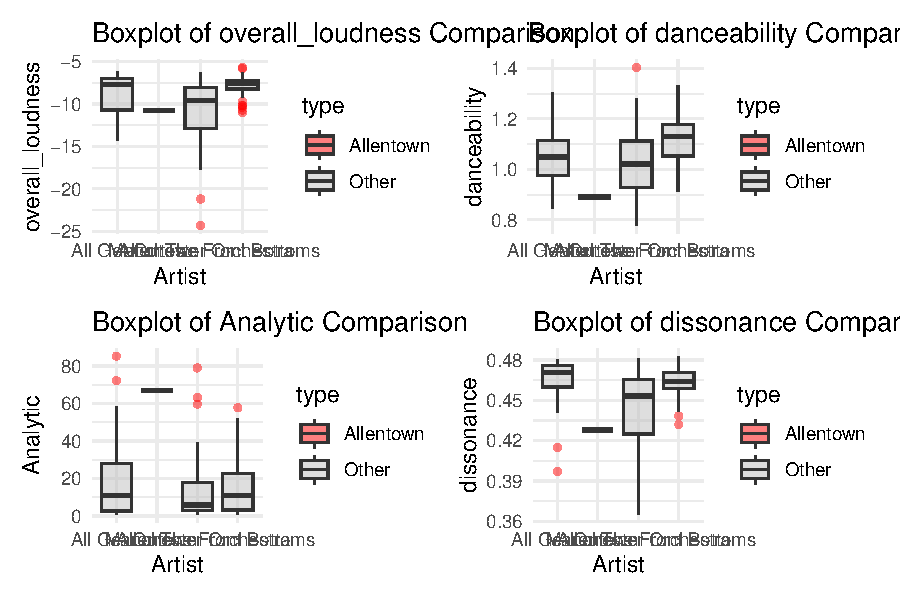
\includegraphics[width=\maxwidth]{figure/boxplot_plots-1} 
\end{knitrout}
  
  \newpage  % Create a page break for the next section

\subsection{Average Comparison for Select Features}
Here’s the comparison of the average feature values for each artist and "Allentown":

\section{Feature Comparison of Artists}

The following plots compare the average values of various features across different artists.

\begin{knitrout}
\definecolor{shadecolor}{rgb}{0.969, 0.969, 0.969}\color{fgcolor}\begin{kframe}


{\ttfamily\noindent\bfseries\color{errorcolor}{\#\# Error: object 'features\_to\_compare' not found}}

{\ttfamily\noindent\bfseries\color{errorcolor}{\#\# Error: object 'feature\_plots' not found}}

{\ttfamily\noindent\bfseries\color{errorcolor}{\#\# Error: object 'final\_avg\_plot' not found}}\end{kframe}
\end{knitrout}

\section{Discussion}
As seen in the figures above, there is no definitive answer between the artists, Manchester Orchestra, All Get Out, and The Front Bottoms. The charts show however that the averages and data for the selected features fit best with Manchester Orchestra suggesting that they are the band that contributed most to the song. 

\begin{tiny}
\bibliography{bib}
\end{tiny}


\end{document}
